\section*{Discussion}

\subsection*{Comparison with other methods}
\subsubsection*{Paragraph about hybrid models}

Our approach is an original application of Bayesian multilevel modelling, and can be considered a logical extension of other Bayesian approaches developed to deal with processes that occur at multiple scales and using several models simultaneously. 
In particular, this development has certain similarities with Bayesian model averaging, Bayesian calibration of process-based models and hierarchical Bayesian modeling. 
Bayesian model averaging aims to combine several alternative models to obtain better predictions while taking into account parameter uncertainties \citep{Hoeting1999}, and has been applied numerous times in ecology where the mechanisms underlying a complex phenomenon are often unknown \citep[e.g.][]{Wintle2003, Link2006}. 
Bayesian model averaging considers models operating at the same scale and the posterior distribution is usually determined with Gibbs sampling. 
Bayesian calibration of process-based model focuses on uncertainty of the parameter values in the process-based models, in this case the values of the parameters are calibrated by the model output \citep{VanOijen2005, VanOijen2011}. 
In contrast with the Bayesian model averaging and calibration techniques, our approach handles data and models operating at different hierarchical scales, and uses process-based models to constrain the shape of a generally more correlative meta-model.
Similar hierarchical approaches have been applied to diverse fields, including engineering \citep{Booth2013}, hydraulic conductivity models \citep{Dostert2009, Efendiev2005, Efendiev2005a}, plant physiology \citep{Ogle2008, Ogle2009}, and climate and atmospheric modelling \citep{Zimmerman2005, Mcmillan2010, Kang2012}.

\subsection*{Advantages of Model Integration}
Models are important tools that are being increasingly used by land managers to face challenges associated to decision-making. 
A growing number of models are available, but they can provide diverging answers to very similar questions, due to the differences in their assumptions and methodology. 
This can create confusion and even some mistrust towards models, and as a consequence some managers may be discouraged to incorporate any model at all in their management plans. 
By integrating different types of models---and their outputs---into a common framework, we believe that our approach can contribute to overcome the gap between modelers and practitioners and thus to promote a widespread use of models to support decision-making.

Our approach also allows for a clear, transparent identification of uncertainties and how they are transmitted throughout the modelling process. 
This is one of the main strengths of this approach, and offers several advantages. 
For instance, transparency in uncertainty can be considered as a sort of sensitivity analysis, in which areas with large uncertainty can be detected and new experimental research or additional data collection can be designed (e.g., Example 1, Figs. \ref{fig:ex1_sampling}, \ref{fig:ex1_precip})
The new knowledge resulting from this research can be readily incorporated into the metamodel, allowing for an iterative learning process that will undoubtedly contribute to reduce uncertainty in predictions for a wide range of environmental conditions. 
Moreover, our framework embraces change as a fundamental process and is able to adapt and respond to it. 
The ease of incorporation of new knowledge to the modeling framework (including new theory or the result of management and experimental efforts), will allow for a rapid adjustment of the predictions and the incorporation of the most recent available knowledge into management plans. 
In an era of continuous and unprecedented change, adaptive approaches such as the one presented here are often highlighted as a pressing need in order to develop strategies to promote ecosystems that are both feasible and resilient \citep[][Fig. \ref{fig:adaptive_management}]{Seastedt2008, Mori2013}.

%==================
% FIGURE

\begin{figure}[tb]
	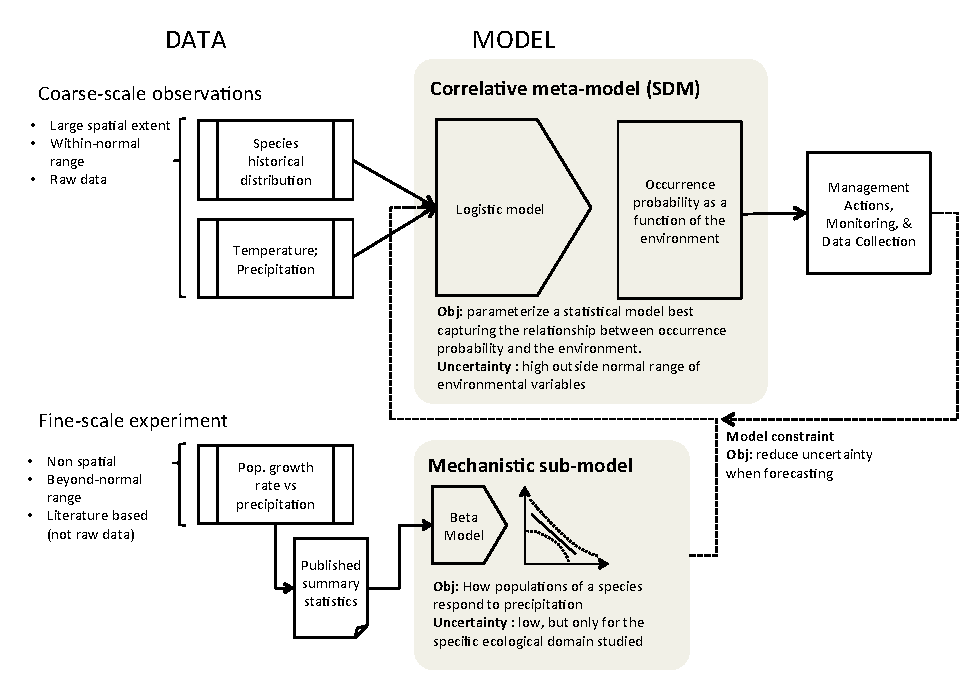
\includegraphics{adaptive_management.pdf}
	\caption{Sample workflow for applying the models presented in the first example in an adaptive management context.
	Critical steps include specifying the meta-model, identifying additional sources of information to be used as constraints on the meta-model, then using the integrated prediction for decision-making.
	As additional information becomes available from monitoring the results of management, this information can be incorporated in additional sub-models to further refine the meta-model.}
	\label{fig:adaptive_management}
\end{figure}

% ERUGIF
%==================


\subsection*{Challenges} 
Although our approach is highly flexible and can be applied in a number of situations, there are some challenges to successfully using the framework.
As with any modelling effort, good model specification with strong links to theory are essential \citep{Austin2007}.
Poorly specified models will produce outputs that are uninformative or misleading, and model integration is not a cure for these problems.
In the worst case, constraining a meta-model with a poor sub-model can result in outcomes that are worse in terms of bias and uncertainty than those produced by a naive model.
We expect model selection will play an important role in applications of our framework, and such schemes can be incorporated relatively easily \citep{Madigan1995, Wasserman2000, Tenan2014}.

In a similar fashion, the quality and availability of data imposes a significant constraint on the number and type of models that can be implemented.
The capacity to implement a model is very low if data requirements are prohibitive. 
Adequate coverage of explanatory variables is a significant obstacle, and exploratory analyses can be a significant aid in understanding how data coverage impacts resulting predictions \citep{Mckenney2002}.
Integration can ameliorate these issues to some extent by using supplemental information (and conceptual advances) in additional sub-models where coverage is weak (e.g., Example 1, Figs. \ref{fig:ex1_precip}, \ref{fig:ex1_map}).
For example, \citet{Freckleton2009} estimated that data is too scant to successfully develop highly mechanistic models predicting weed population numbers. 
A strong asset of our proposed method is that it can be used without the full suite of data that would be required to run a fully mechanistic model. 
Since the meta-model is correlative, the rough structure of our approach only needs e.g. presence-absence data to be effective. 
Then any additional mechanistic data that is available will enhance predictions by constraining outputs of the meta-model. 

Finally, determining the functions to use to express the likelihood of the sub-models given the meta-model (i.e., Eqs. \ref{eq:ex1_integrated}, \ref{eq:integrated2}) will remain a significant challenge.
We have shown in our examples that even simple scaling functions can provide reasonable constraints on the meta-model. 
However, it is likely that with very large differences in scales (e.g., comparing cellular processes to landscapes), simple functions will be inadequate, requiring more traditional upscaling methods that combine explicit processes with additional data (and, necessarily, additional parameters) before meaningful model integration will be possible.

\subsection*{Applicability of the method}
\defcitealias{TERN2013}{TERN, 2013} %% this is needed to make the organizational citation in the following paragraph work correctly
Integrated approaches have gained momentum in recent years, with integrative science being featured as a central theme for several science-based governmental organisations around the world \citep[e.g.][\citetalias{TERN2013}]{Bernier2013}. 
Incorporating information from multiple sources, particularly with respect to uncertainty,  fosters a connection between scientifically-generated knowledge and policy, and is therefore an important tool for adaptive management \citep[][Fig. \ref{fig:adaptive_management}]{Rehme2011}.
Such approaches are needed in formulating management plans for vulnerable species and ecosystems to avoid basing decisions on too-narrow subsets of the available information \citep{Dawson2011}.
The flexibility of our approach may also represent an advantage for management by easing the integration of specific decision making criteria (e.g. desired grain and extent of outputs) into model development. 
Successful use of an integrated modelling approach will always remain dependent on an intimate understanding of the decision-making process by modellers, emphasizing the importance of close collaboration between with practitioners at all stages of model development \citep{Guisan2013}.

The transparency of our approach is also a clear advantage. 
To be useful, models should be transparent analytical tools, not black boxes \citep{Addison2013}. 
A key criteria for model applicability is the explicit and detailed communication of specific model objectives, characteristics, limits, and uncertainties, as well as its ecological foundation \citep{Guisan2013}.
Integrating submodels allows for clear specification of desired model outputs (via the specification of the metamodel) while easily retaining important ecological objectives (via careful specification of submodels).
Insufficiently documented models are difficult to assess in real world situation, and therefore only having limited relevance  for decision support \citep{Guisan2013}.
Model workflow documentation becomes more crucial in the case of integrated modelling approaches, which incorporates information from various scales and resolutions within a number of aggregated sub-models. 
A transparent and well documented workflow describing the process of model integration ensures reproducibility and facilitates its use in an applied context (Fig. \ref{fig:adaptive_management}). 
The issue of uncertainty also limits the use of models in guiding decisions. 
Model outputs are considered too uncertain for decision-making \citep{Addison2013}. 
The transparent estimation of the uncertainty provided by this modelling approach may be a significant advantage. 

\subsection*{Accessibility}
Results of models predicting species ranges are increasingly used by resource managers, conservation biologists, or forest ecologists for formulating or adjusting recommendations. 
The utility of such models depends on their ability to help evaluate events beyond the bounds of the available data, including in future situations constrained by climate change. 
In this context, practionners judge model usefulness on two criteria : Does the model provide reliable predictions at the needed time and space scales, and can the model be implemented given the available data and technical expertise? 
Since most decision makers work at local space scales and follow specific time frames, modelers face the obvious challenge of providing detailed outputs while preserving implementation capacity.
In terms of model outputs, our framework is transparent in terms of uncertainty by virtue of providing easily interpretable probability distributions for model parameters and predictions.
However, developing the models requires careful model specification, knowledge of applied Bayesian methods, and, in some cases, extensive programming.
In many cases, off-the-shelf software \citep[e.g.,][]{R, RJAGS} can adequately express the model likelihoods with minimal programming, but more complicated models will require the development of custom software.
Thus, this framework will require significant investment in developing customized code for the samplers in order to actually estimate parameters.
No doubt, the implementation of our proposed method is currently too technically challenging for most practionners. 
However, the same was true of all statistical techniques or modeling approaches when they were initially developed. 
In addition, some of the computation costs that were associated with many techniques have now vanished, and even the conceptual challenges associated Bayesian statistics are being reduced as they gain popularity in the scientific literature. 
We therefore argue that our proposed approach as a strong potential for direct use in our real world where climate is quickly changing and conservation practices must be adjusted accordingly.

\subsection*{Future directions}
\begin{itemize}
	\item incorporation of spatially explicit models into the framework? \citep[e.g.,][]{Fortin2012}
	\item more sophisticated meta-models (e.g., state-transition models)
	\item others?
\end{itemize}
